\section{Fault Detection and Diagnosis} 
\label{sec:system_char}

%\hl{show that there is behavior is amenable to learning, fearures are there to be learnt -- Sibin} 
%\ashish {Added section above.}

In \S\ref{sec:aout_char}, we analyzed the impact of failures on the characteristics of the \aout output signal in both time domain and in frequency domain using FFT. We now investigate if the characteristics of \aout contain behavior that is amenable to learning \ie if there are features to be learnt. First, we analyze the learnability of the fault detection and diagnosis problem in \S\ref{subsec:learnability}. During this, we show that in every type of failure, there exists information about the failure and quantify the difference in physics captured by FFT coefficients using a K-S statistic test~\cite{massey1951kolmogorov}.

\begin{wraptable}{L}{0.4\textwidth}
	%\begin{table}5
	%\setlength\tabcolsep{1.45pt}
	\setlength\tabcolsep{2.5pt}
	%\minipage{0.75\textwidth}
	%\footnotesize
	\centering
	%\small
	%\hrulefill
	\caption{{K-S Statistic Results}: FC1 -- FC5 : Failure Class I -- V. W : working sensor.}
	%\resizebox{\textwidth}{!}{
		%\begin{tabular}{p{2.25cm}p{14.5cm}}
		%\begin{tabular}{p{2cm}p{3.5cm}p{3cm}p{2cm}}
		\begin{tabular}{l c c c c c c}
			\hline
			\textbf{Failure} & \textbf{FC1} & \textbf{FC2} & \textbf{FC3} & \textbf{FC4} & \textbf{FC5} & \textbf{W} \\
			\hline \hline
			K-S Test & 0.41 & 0.33 & 0.49 & 0.65 & 0.95 & 0.09 \\
			\hline 
		\end{tabular}
		%}
	\label{tbl:ks_test_results}
	%\end{table}
\end{wraptable}

\subsection{Learnability of the Analysis}
\label{subsec:learnability}

We performed a 2-sample Kolmogorov–Smirnov (K-S) statistic test~\cite{massey1951kolmogorov} to validate our hypothesis that the \aout distributions from both working and failed sensors are different.  We performed the tests at a significance level ($\alpha$) = 0.05, that results in a K-S statistic threshold of 0.1 -- a standard threshold for checking if sample differences in two distributions imply difference in population. {\bfseries Table~\ref{tbl:ks_test_results}} shows the K-S statistic (\texttt{kstest2} in Matlab~\cite{mathworks2015kstest2}) computed for each class of failure relative to a working sensor in columns FC1 -- FC5. We make the following observations :

\noindent \textbf{Failed sensors have different frequency characteristics compared to a working sensor:} Each failure class FC1 --- FC5 has a K-S statistic value > 0.1 when compared to a working sensor (W), indicating that the distributions of faulty and working sensors differ. %This shows the presence of information to be learnt about each type of failure not present in a working sensor. 

\noindent \textbf{The worse the failure, higher the K-S statistic:} A sensor with oil condensation on the lens (C4) (a more pernicious fault leading to missed obstacles) resulted in a K-S statistic of 0.65 compared to 0.33 for a sensor with lens deformation (C2) (milder fault resulting in some blind spots). The K-S statistic captures the divergence between physics of failed and working sensors.


\noindent \textbf{Working sensors have similar characteristics:} We performed a sanity check between distributions of multiple working sensors and noticed the consistency among them in the frequency domain. Computing the K-S statistic resulted in a value below the 0.1 threshold implying similar physics as seen in {\bfseries Fig.~\ref{fig:normal_normal_freq}}.
%the \aout distributions show similar characteristics are drawn from the same source 


% We observed that the K-S Test (kstest2 in Matlab~\cite{mathworks2015kstest2}) computed to a logical 1 in each of the failed cases implying that the behavior of a working sensor is clearly distinct from a failed sensor.

\noindent \textbf{Summary:} K-S test shows the possibility of information that can be extracted to generate a physics-based reliability feature vector for the PIR sensor. This also motivates using classification techniques to identify the information difference between different failure scenarios~\cite{breiman2001random,cunningham2020k}.

%\begin{wraptable}{R}{7.5cm}%[ht]\small
%	%\renewcommand{\arraystretch}{1.1}
%	\centering
%	\footnotesize
%	% \vspace{-5pt}
%	\caption{Some of the features used to analyze the classification between faulty and working sensors}
%	%\centering
%	\begin{tabular}{p{2.5cm} p{4cm}}
%		\hline %\\                   
%		\textsc{\bfseries Feature} & \textsc{\bfseries Definition}\\
%		\hline\hline
%		%\rowcolor{gray!20} \multicolumn{2}{l}{\bfseries Lens Subsystem}\\
%		\rowcolor{gray!20} Fourier Coefficients & Uses FFT algorithm to calculate frequency spectral coefficients\\
%		Autocorrelation & Finds repeating patterns or missing fundamental frequencies in a signal \\
%		\rowcolor{gray!20}Lempel-Ziv (LZ) Complexity & Calculates number of entries needed to encode the time series for LZ compression\\
%		Wavelet Transform & Calculates Wavelet coefficients using Mexican Hat Wavelet \\
%		\rowcolor{gray!20}Number of Peaks & Calculates the number of peaks considering 'k' neighbours\\
%		Sample Entropy & Quantifies the amount of regularity and unpredictability of fluctuations\\
%		\hline
%	\end{tabular}
%	\label{tab:tsfresh_features}
%	%\vspace{-5pt}
%\end{wraptable}
%%%%%%%%%%%%%%%%
% Shapley Summary
%%%%%%%%%%%%%%%%
\begin{figure}
    \begin{subfigure}[t]{0.45\textwidth}
		\centering
		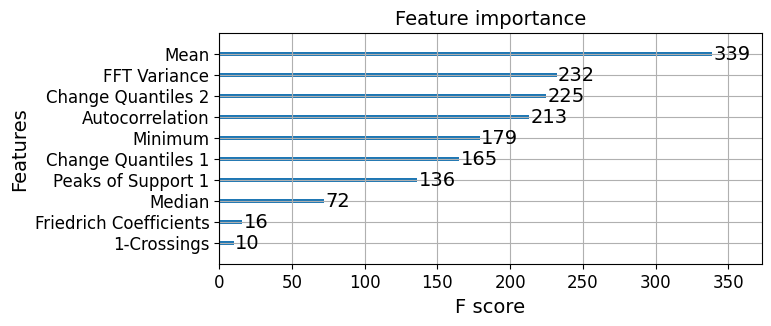
\includegraphics[width=\textwidth]{figures/classification/BH/BH-feature-selection.png}
        \caption{}
        \label{fig:BH_feature_selection}
    \end{subfigure}
    \hfill%
    \begin{subfigure}[b]{0.49\textwidth}
        \centering
        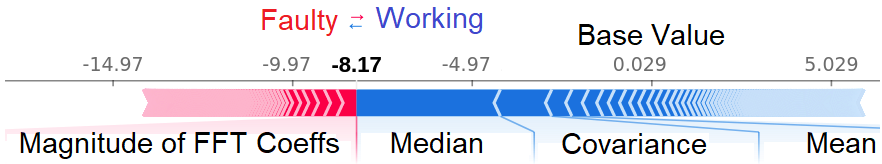
\includegraphics[width=\textwidth]{figures/classification/shapley/shap_expected_4.png}
        \caption{}
        \label{fig:shapley_summary}
    \end{subfigure}
    \caption{\ca Top 10 features selected using B-H procedure, \cb Summary of Shapley Values showing FFT coefficients separate faulty and working classes.}
\end{figure}
%%%%%%%%%%%%%%%%
% End of Shapley Summary
%%%%%%%%%%%%%%%%

% \hl{NEW -- B-H}
\subsection{Feature Selection and Importance} 
\label{subsec:bh} 
We use both the time domain and frequency domain features of the \aout signal to classify the sensor to either working or one of the faulty classes. As the number of features that can be derived is huge (\eg in our case 305), we use the Benjamini-Hochberg (B-H) feature selection algorithm ~\cite{benjamini1995controlling} to estimate and analyze \textit{feature importance} in the \aout collected for working and each class of faulty sensors.

B-H technique is used offline with training data to decide which features are useful in predicting the label of the sensor (\eg working vs. class X). The output of B-H feature selection process is a \textit{feature importance score (F-score)} that indicates how useful or valuable each feature is in the decision making process. The higher the F-score, the more important the feature is to prediction. 

B-H feature selection process works by initially training an ensemble of decision trees on all features, derived from both time and frequency domain features as mentioned in Christ~\etal~\cite{christ2018time} and implemented in the open source library \texttt{tsfresh}~\cite{tsfresh2018code}. It then measures the prediction accuracy using every feature. This gives a high accuracy at the expense of overfitting. Thereafter, each feature vector is independently evaluated with respect to its significance for prediction using hypothesis testing, assigning it a F-score. It then iteratively prunes features having low F-scores, trains decision trees using these reduced features and measures prediction accuracy. The process stops when a user-set threshold of accuracy is met or when all the combinations have been tested. 

Applying the B-H process to our training data containing both faulty and working sensors, \emph{we pruned 305 features for our entire data set to obtain 10 features at a slightly better accuracy}. The larger set of features are derived from the list of features in {\bfseries Table~\ref{tbl:feat_list}}. \texttt{tsfresh} attempts to identify the strongly and weakly-relevant features in the fault detection and diagnosis process. It uses an algorithm named \texttt{fresh} (`FeatuRe Extraction based on Scalable Hypothesis'), that has been shown to be an efficient, scalable feature extraction technique used in early stages of ML pipelines~\cite{christ2016distributed, christ2018time}. \texttt{fresh} uses a 3-phase technique to select significant features while controlling the percentage of irrelevant features. First, \texttt{fresh} characterizes the time series using the larger set of features, some of which are indicated in {\bfseries Table~\ref{tbl:feat_list}}. Note that the complete feature set is comprehensive and also includes composite features derived from the simple features. In the second step, each feature vector is individually and independently evaluated with respect to its significance using hypothesis testing. As a part of the hypothesis testing, the significance of each feature is quantified into a p-value, with smaller p-values indicating that the feature is not statistically significant. In the third and last step, the feature vector is evaluated using the B-H process to decide which features to keep -- by transforming the hypothesis testing scores into F-scores. This step ensures that incorrectly rejected features are regulated while conducting multiple hypothesis tests. {\bfseries Fig.~\ref{fig:BH_feature_selection}} plots the F-score for the selected 10 key features in both time and frequency domains. These include: \ca FFT Variance that indicates how spread the frequency distribution is, \cb Autocorrelation that generalizes periodicity or patterns in the time domain, and \cc  Measures of central tendency such as mean, median and change quantiles that measure the time domain changes within a corridor. This process is performed offline and the significance of the pruned feature set is guaranteed by the B-H algorithm. Note that both Friedrich coefficients and Peaks of support capture short term dynamics of the signal. The mathematical definition of these features can be found in statistics textbooks and implementations in the \texttt{tsfresh} GitHub repository~\cite{tsfresh2018code}. We can continue the feature pruning process by training decision trees on combinations of features from these 10 features and measuring prediction accuracy. We stopped the feature pruning with 10 features since we consistently obtained an accuracy of 97-99\% in practice with this smaller set of features.%There are additional features such as Friedrich coefficients and Peaks of support, the definitions of which can be found in statistics textbooks.


\begin{table}
%\begin{wraptable}{R}{0.65\textwidth}%[ht]\small
%\renewcommand{\arraystretch}{1.1}
%\vspace{-\baselineskip}
	\centering
	\footnotesize
    \caption{Features before pruning, calculated using the \texttt{tsfresh}~\cite{tsfresh2018code} library. \texttt{tsfresh} uses hypothesis testing to prune and select most significant features.}
    \begin{tabular}{p{2.25cm} p{12 cm}}
    \hline %\\
    \textsc{\bfseries Feature} & \textsc{\bfseries Description}\\
    \hline\hline
    %\rowcolor{gray!20} \multicolumn{2}{l}{\bfseries Computational}\\
    \rowcolor{gray!20} abs\_energy & Absolute energy \ie sum of squares   \\
    agg\_autocorrelation & autocorrelation of the time series \\
    \rowcolor{gray!20} agg\_linear\_trend & linear least-squares regression aggregated over chunks versus the sequence from 0 up to (number of chunks - 1) \\
    approximate\_entropy & vectorized approximate entropy \\
    \rowcolor{gray!20} c3 & c3 statistics to measure non linearity \\
    binned\_entropy & calculates entropy over a set of equidistant bins \\
    \rowcolor{gray!20} energy\_ratio\_by\_chunks & the sum of squares of chunk expressed as a ratio with the sum of squares over the whole series \\
    fft\_aggregated & the spectral centroid (mean), variance, skew, and kurtosis of the absolute fourier transform spectrum \\
    \rowcolor{gray!20} fft\_coefficient & the fourier coefficients of the one-dimensional discrete fourier transform \\
    fourier\_entropy & the binned entropy of the power spectral density of the series \\
    \rowcolor{gray!20} friedrich\_coefficients & Coefficients of polynomial fitted to the Langevin model \\
    linear\_trend & a linear least-squares regression for the values of the series versus the sequence from 0 to length of the time series minus one \\
     \rowcolor{gray!20} number\_peaks & the number of peaks of at least support n \\
    root\_mean\_square & the root mean square (rms) of the series \\
     \rowcolor{gray!20} number\_crossing\_m & the number of crossings of series across m \\
    sample\_entropy & sample entropy of the series \\
     \rowcolor{gray!20} variation\_coefficient & the variation coefficient (standard error / mean, give relative value of variation around mean) of the series \\
    ratio\_beyond\_r\_sigma & ratio of values that are more than $r$ standard deviations away from the mean \\
     \rowcolor{gray!20} others & mean, variance, quantile, mean absolute change and so on \\
    \hline
    \hline
    \end{tabular}
    \label{tbl:feat_list}
    %\vspace{-15pt}
    %\vspace{-\baselineskip}
%\end{wraptable}
\end{table}

%We can continue the feature pruning process by training decision trees on combinations of features from these 10 features and measuring prediction accuracy. We stopped the feature pruning with 10 features since we consistently obtained an accuracy of 97-99\% in practice. 

%Applying the B-H process pruned the number of features to  the relative importance of the various features that distinguish working from faulty sensors. 

%We performed B-H feature selection on our training dataset comprising working and faulty sensors. The F-score for various features is shown {\bfseries Fig.~\ref{fig:BH_feature_selection}}.  Note that {\bfseries Fig.~\ref{fig:BH_feature_selection}} consists of features both in the time domain as well as the frequency domain. 

%\ashish{order of importance, actual number}
%The relative importance of features learnt by the model to predict the label of a sensor can vary from one deployment to another -- but the approach of using BH procedure to find relative importance of features followed by using SHAP values is general in nature. The end-goal is to find definitive features that can characterize the intrinsic signal, either in time and frequency domain. The features learnt by the model can vary from one building to another.

\subsection{Monitoring Feature Performance using Shapley Additive Explanations (SHAP)} \label{subsec:shap} Once the important features are identified using the B-H feature selection process, we use the technique of SHAP~\cite{NIPS2017_8a20a862} values to \textit{explain or interpret} the output of a prediction. SHAP uses game-theoretic techniques to explain how the output of a prediction changes by conditioning on every feature present in the reduced feature set given by B-H process.  


%It assigns each feature an importance value based on its contribution to a prediction. 
%Quantitatively, it explains how the output of a prediction changes conditioning on a feature. 
%\ashish{shap value quanlitatively is used to interpret the behavior of the feature rather than the quantitiatively, direction of contribution}

%\ashish{how each feature is afftecting in the prediction using game theory. Model is strategy. Player are features.}

{\bfseries Fig.~\ref{fig:shapley_summary}} shows an example of how SHAP values are analyzed for a particular prediction on a classification between faulty and working sensors. The features in red contribute to the sensor being predicted as faulty, whereas the features in blue contribute to the sensor being predicted as working. As seen, the competing features that contributed to this decision are the FFT coefficients and the statistical features~\viz mean, median and covariance. 
%the shows a plot of the relative importance of different features in faulty and working sensors.
In this prediction, the FFT coefficients push the prediction to that of a faulty sensor while the mean, median and covariance push the prediction to a working sensor. The base value is the average SHAP value output by the model for the entire training dataset, and the value in bold is the SHAP value for this particular prediction. We leverage an open-source library implementation of the algorithm from Lundberg~\etal~\cite{NIPS2017_8a20a862, shap_implementation} that sorts the features by sum of SHAP value magnitudes over all the samples and conditionally rejects the feature contributing lowest to the prediction. Thus, we use the feature explanations from SHAP values to tune the model performance. %adaptively improve the prediction performance in deployment by analyzing what features are contributing to predictions.

\subsection{\sol: Fault Detection \& Analysis Algorithm}
\label{subsec:high_level_algorithm}
%We now present our algorithm \sol towards fault detection in PIR sensors. 
We now combine the insights gathered from physics and machine learning techniques to develop a unified algorithm, called \sol, that is deployable at the edge, to isolate and diagnose faults.
\sol consists of 2 stages: \ci pre-deployment (training) stage, wherein the reference \aout values for a set of sensors (both working and faulty) are collected offline and analyzed to extract key features and \cii deployment stage, wherein the features from a operational \aout signal is matched with the previously extracted features in order to detect and isolate faults. We next describe both the stages in detail.
%\ashish{Not requireing complex ML algorithms.}

%%%%%%%%%%%%%%%%
% PRE-DEPLOYMENT, DEPLOYMENT STAGES
%%%%%%%%%%%%%%%%
\begin{figure}
	\begin{minipage}[t]{0.26\textwidth}
		\centering
		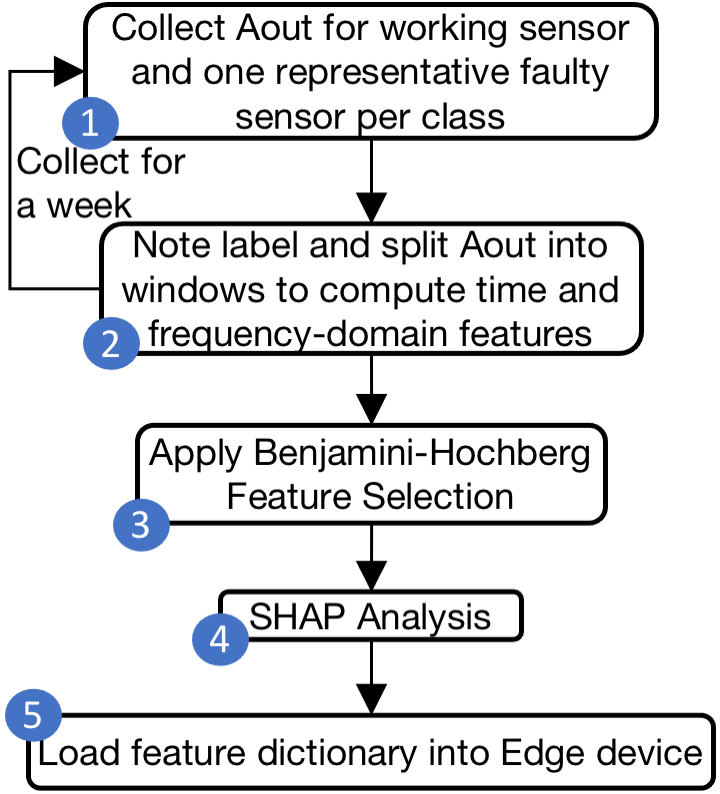
\includegraphics[width=0.9\textwidth]{figures/deployment/predeployment-stage-2.png}
		%\vspace*{-1.0\baselineskip}
		\caption{\footnotesize{Pre-deployment stage}.}
		%\vspace*{-0.25\baselineskip}
		\label{fig:pre_deployment_steps}
	\end{minipage}%
	\hfill
    \begin{minipage}[t]{0.22\textwidth}
		\centering
		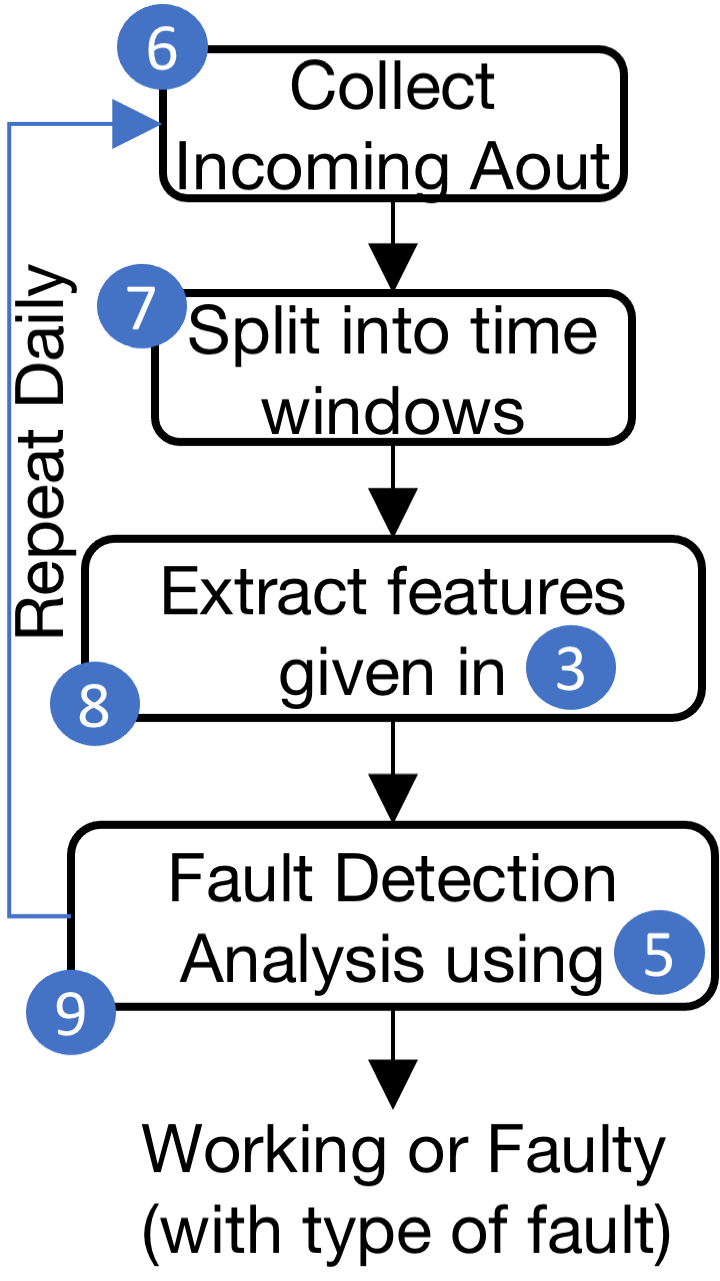
\includegraphics[width=0.7\textwidth]{figures/deployment/deployment-stage-5.png}
		%\vspace*{-1.0\baselineskip}
		\caption{\footnotesize{Deployment stage}.}
		%\vspace{2\baselineskip}
		\label{fig:deployment_steps}
	\end{minipage}
    \hfill
    \begin{minipage}[t]{0.5\textwidth}
        \centering
        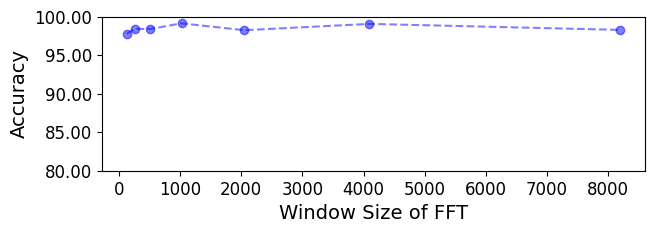
\includegraphics[width=\textwidth]{figures/classification/accuracy_vs_window_size.png}
		\caption{\footnotesize{Model Accuracy} for different window sizes. We choose 1024 as the default window size.}
		\label{fig:accuracy_vs_window_size}
    \end{minipage}
\end{figure}

% \begin{figure}
%     \centering
% 	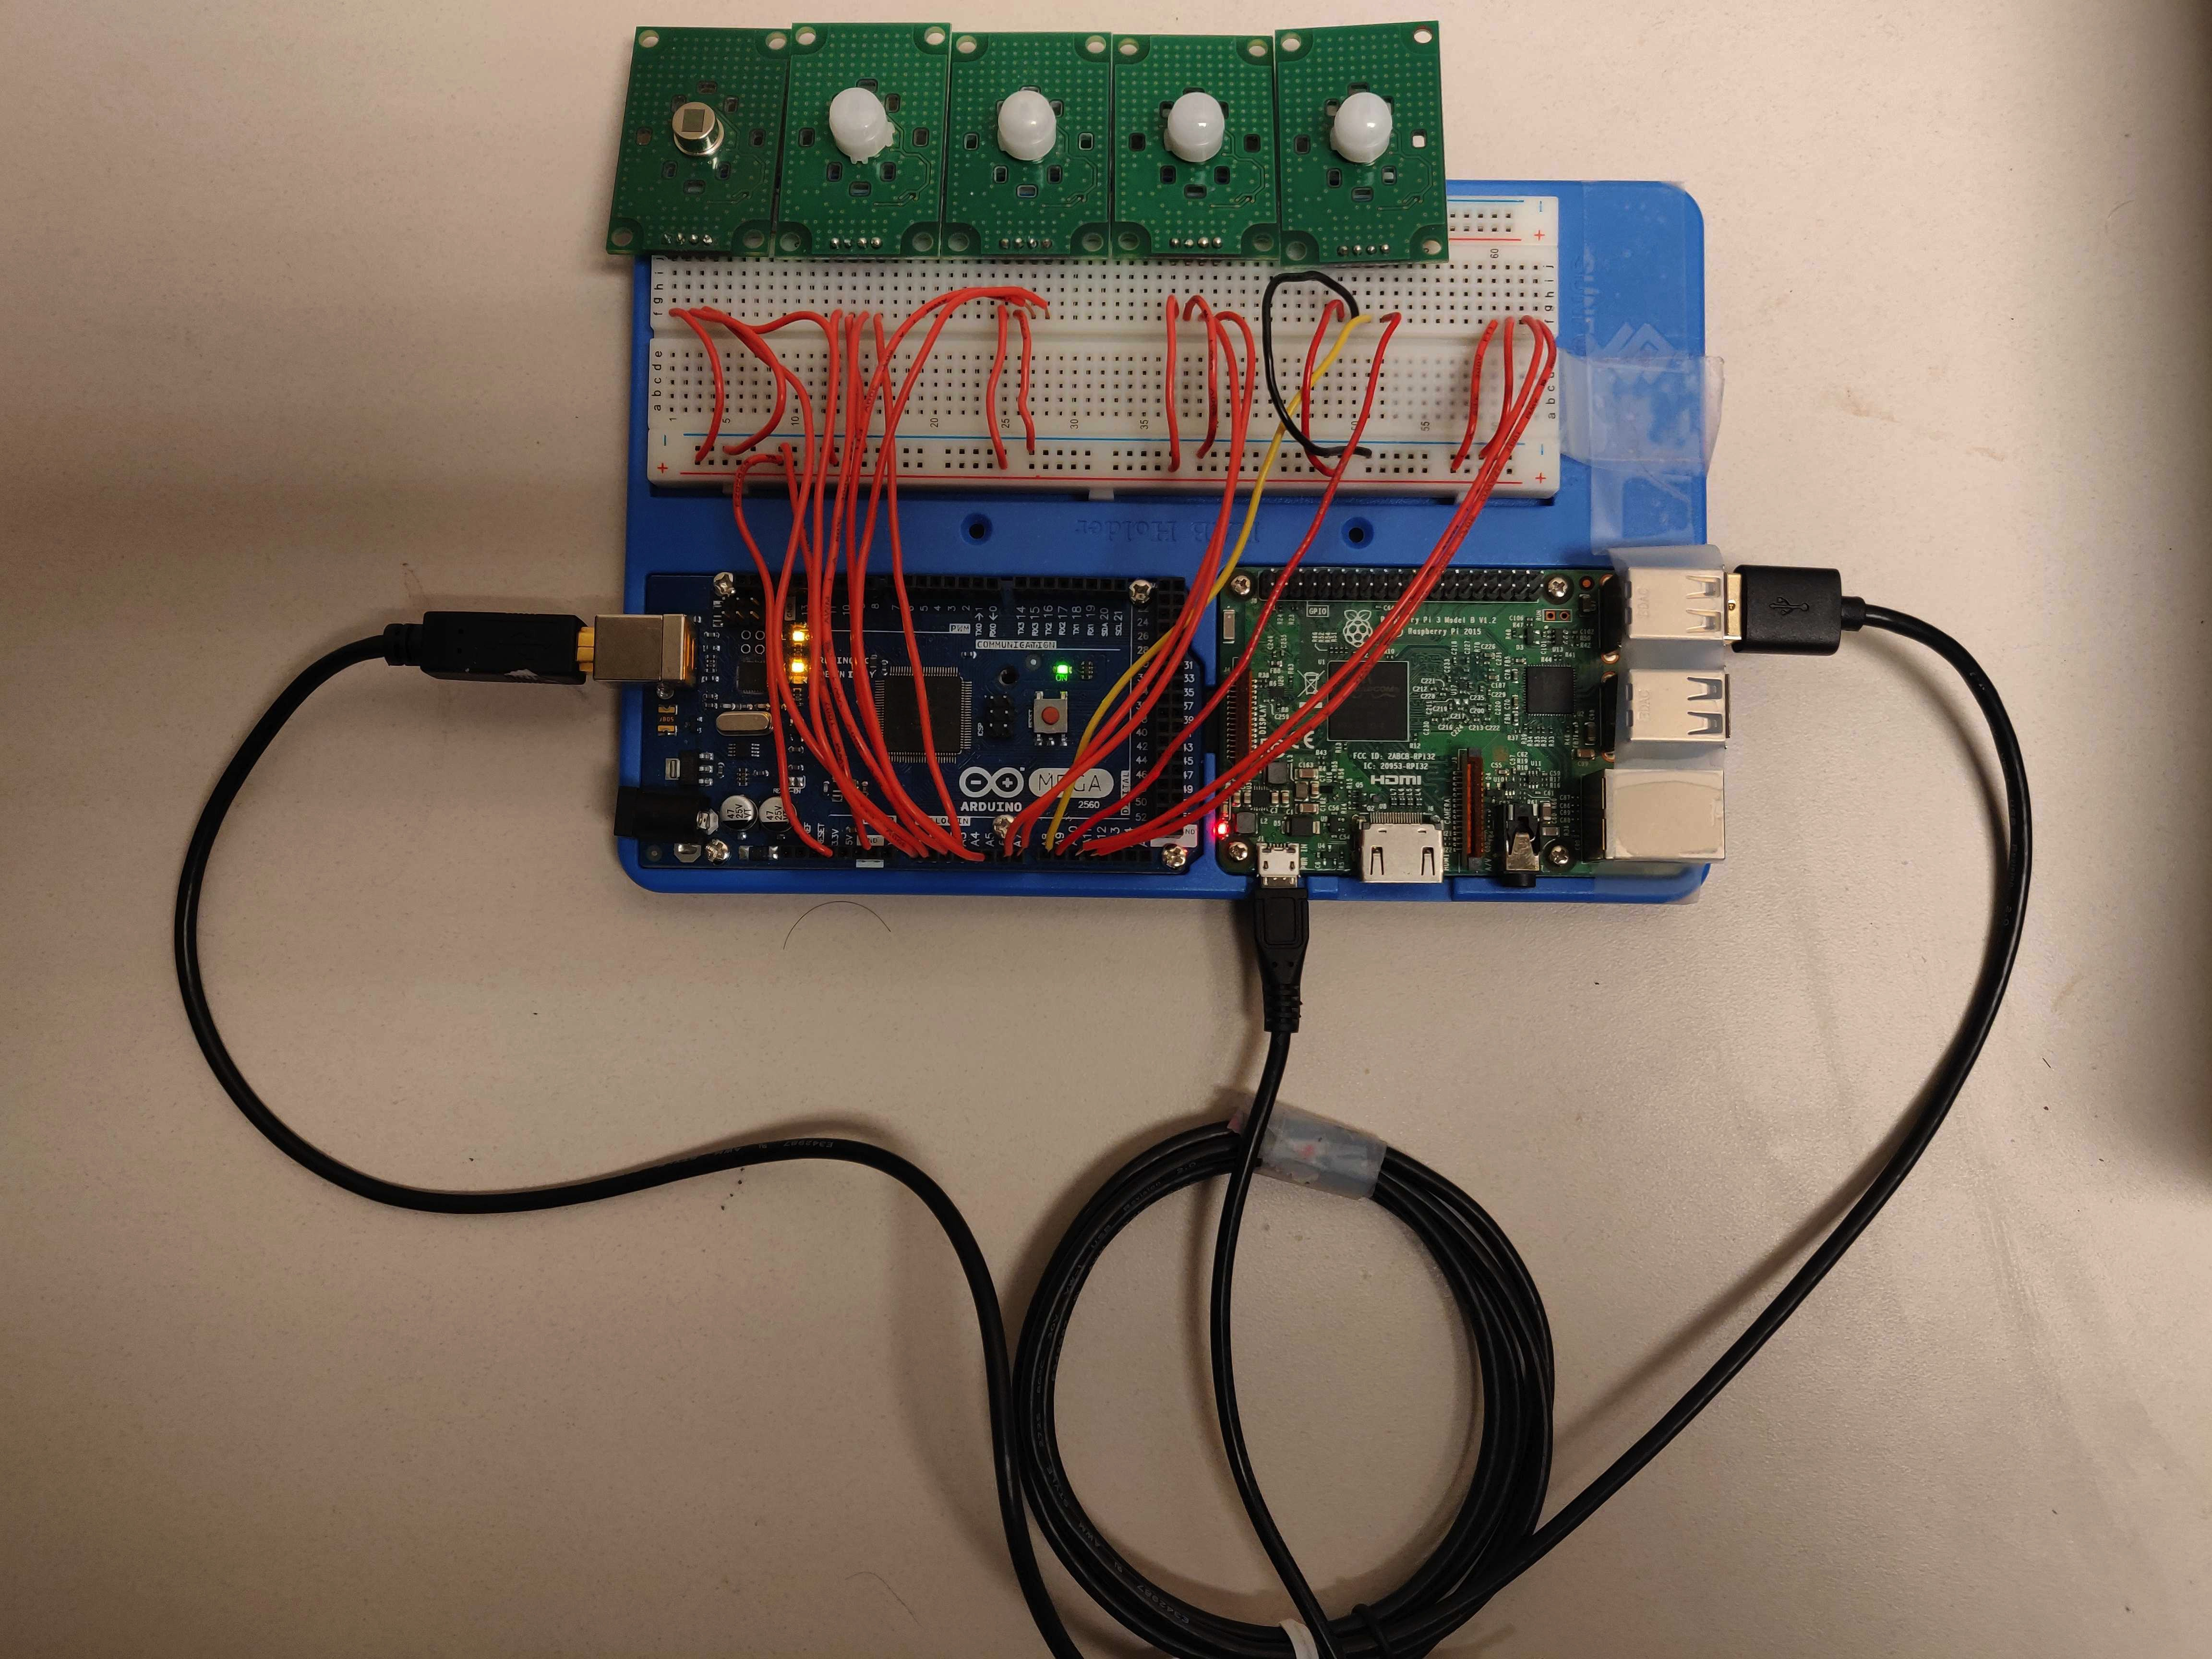
\includegraphics[width=0.22\textwidth]{figures/platform/eval_platform.jpg}
% 	\vspace{-10pt}
% 		\caption{\footnotesize{Edge Platform} used for fault analysis in a PIR sensor.}
% 		\label{fig:platform_photograph}
% 		\vspace{-15pt}
% \end{figure}

% 	\begin{minipage}[b]{0.35\textwidth}
% 		\centering
% 		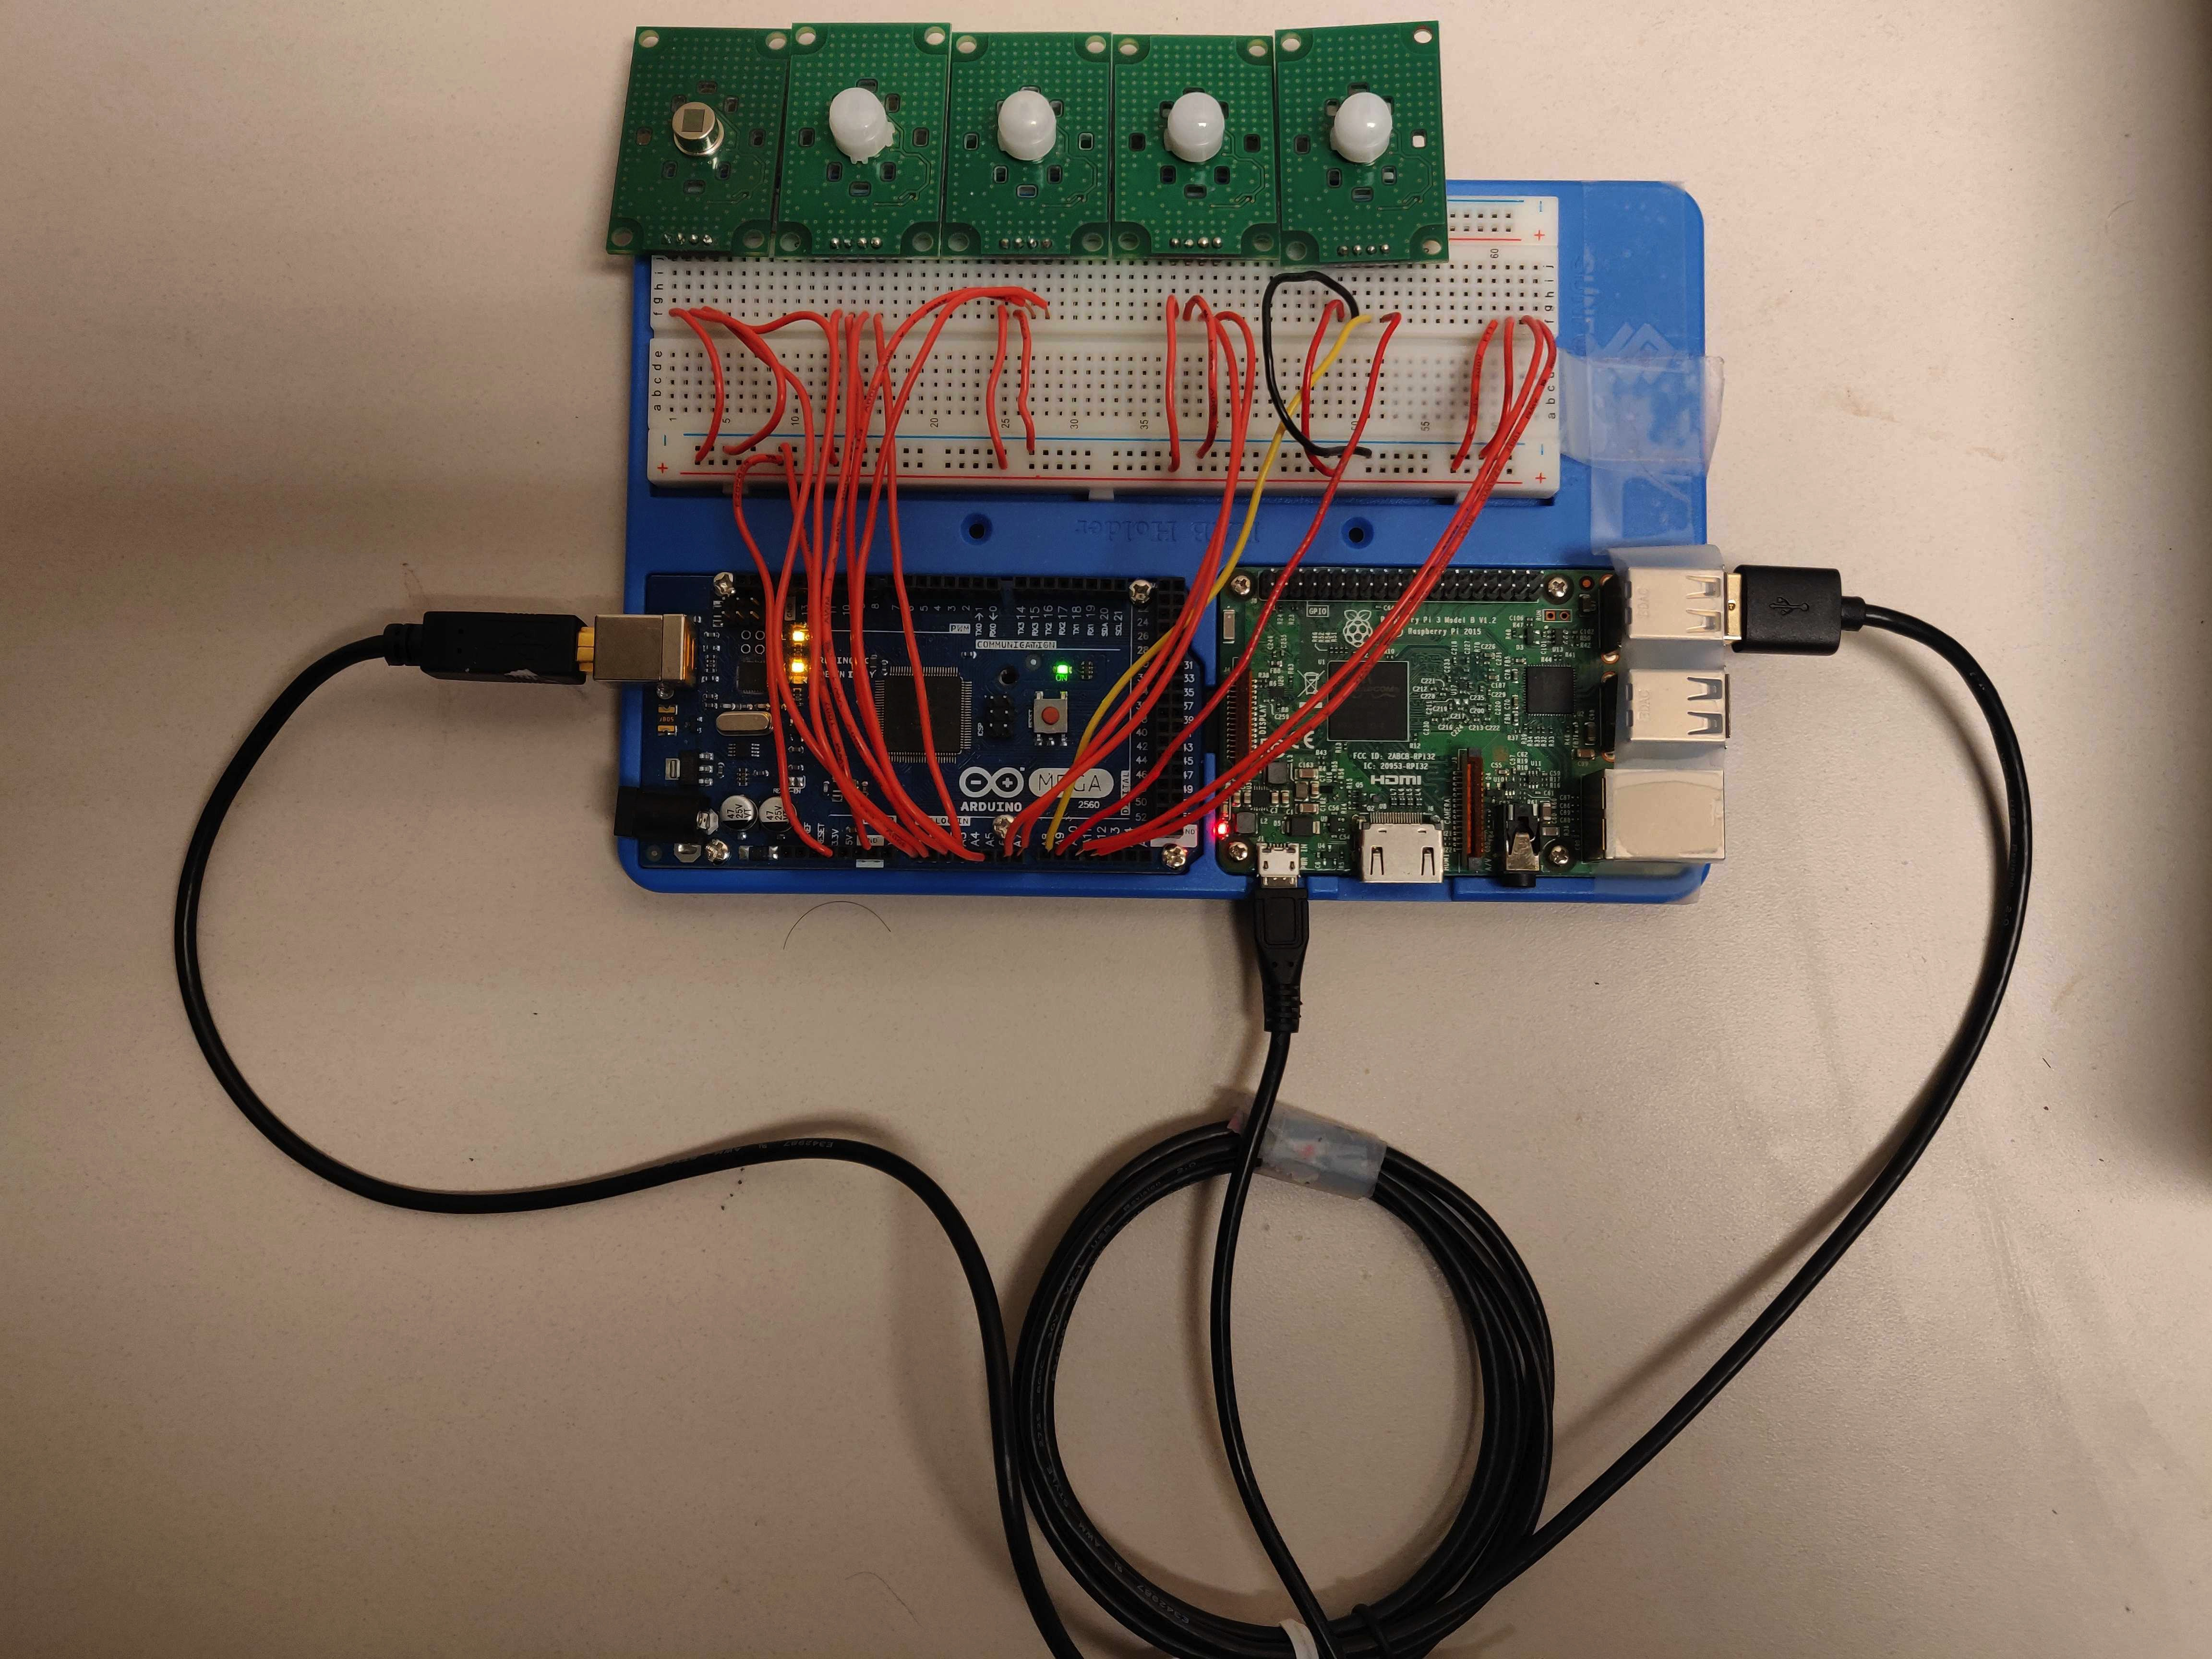
\includegraphics[width=0.6\textwidth]{figures/platform/eval_platform.jpg}
% 		\caption{\footnotesize{Edge Platform} used for capture and analysis of faults in a PIR sensor.}
% 		\label{fig:platform_photograph}
% 	\end{minipage}
% 	\vspace{-10pt}

%%%%%%%%%%%%%%%%
% END OF PRE-DEPLOYMENT, DEPLOYMENT STAGES
%%%%%%%%%%%%%%%%

\subsubsection{Pre-deployment stage} 
\label{sebsec:pre_deploy} 
We first collect \aout from a set of sensors, comprising both working and faulty ones such as the ones shown in {\bfseries Fig.~\ref{fig:pir_sensor_failure_photographs}}. The collected time series data are labeled to form a training dataset. We perform the Benjamini-Hochberg (B-H) feature selection on this dataset to extract key features such as FFT coefficients of \aout for each class of sensor. This forms a feature dictionary containing a smaller number of features along with the failure as a label. We further verify the importance of these features using SHAP analysis and refine the features if necessary.
% We load this feature dictionary into the edge device connected to the PIR sensor.
% that would perform failure analysis during the deployment. 
We then build a classifier model to uniquely identify the sensor failure and load this model into the edge device connected to the PIR sensor. 

We now describe the steps involved ({\bfseries Fig.~\ref{fig:pre_deployment_steps}}):
%
\circled{1} We deploy the working and faulty sensors for a short duration (say few days) in a real-world environment to collect realistic \aout signals for low, medium and high occupancy. 
%
Note that this is a one-time activity performed for a specific PIR sensor type/manufacturer. 
% when installing the sensor, we record the \aout values by deploying it for a duration long enough to capture periods of low occupancy, medium occupancy and high occupancy. %For instance, 
% This stage typically lasted for one week in one of our deployments (university building). 
We used 15 sensors comprising a mix of working and faulty sensors capturing failures in each class as our training set.
%
\circled{2} We note the label of a sensor and split the \aout values into equal-sized time slices (windows) to calculate different time and frequency-domain features. 
%
\circled{3} We apply B-H feature selection process for each type of sensor to identify unique and key features. 
%
\circled{4} We performed SHAP analysis to understand the performance of each feature towards classification and refine them accordingly. 
%
\circled{5} We use the final set of features along with class labels to build a classifier model (we use random forest as our classifier model). This model is then loaded onto the edge devices for fault detection and analysis. We note that while \circled{2} and \circled{3} are computationally expensive, it is acceptable as it is performed offline only once in the pre-deployment.
%\vspace{-5pt}

\subsubsection{Deployment stage} 
This stage consists of the following steps ({\bfseries Fig.~\ref{fig:deployment_steps}}): 
%
\circled{6} First, the operational \aout output signals for the deployed sensors are collected. 
%
\circled{7} We split the \aout into equal-sized windows using same window size as in the pre-deployment. 
%
\circled{8} We extract the necessary features from the \aout signal. 
%
\circled{9} We use a classifier to \ca isolate faulty from working sensors and \cb identify the class of failure in the faulty sensor if applicable. %As mentioned earlier, the pre-deployment stage (to collect features and build a classifier model) is a one-time activity. 
The fault detection (steps \circled{6} - \circled{9}) depends on the application requirements, \ie every hour, day or week. 

%\circled{9} Once the failures are identified, we perform one-time manual verification.
%manually verify the fault detection and analysis. 
% \circled{10} In case of an incorrect decision, the output of the fault detection is analyzed using SHAP values to understand which features drive the decision to mark a sensor incorrectly. We remove that feature from the deployed feature dictionary and perform prediction again. The feature is removed in case the prediction accuracy improves and retained if the prediction deteriorates. This process of feedback from the deployment stage to the pre-deployment stage helps adaptively improve accuracy. The deployment stage is periodic \eg weekly to identify the faulty sensors.

% We extract the FFT coefficients of newly collected \aout data and use a random forest to classify between faulty and working sensors using the FFT coefficients collected in the pre-deployment phase. If the sensor is deemed faulty, we perform further processing on the \aout features of the faulty sensors to identify the nature of fault.


%We load this feature dictionary into the IoT device connected to the PIR sensor that performs analysis in real-time to \ca isolate faulty and working sensors and \cb identify what kind of fault is present in the sensor if applicable.

%\cc We build a classifier model using the above from all working sensors used in the deployment.


%\begin{figure}
%	%%%%%%%%%%%%%%%
%	 B-H FEATURE SELECTION
%	%%%%%%%%%%%%%%%
% 	\begin{minipage}[t]{0.49\textwidth}
% 		\centering
% 		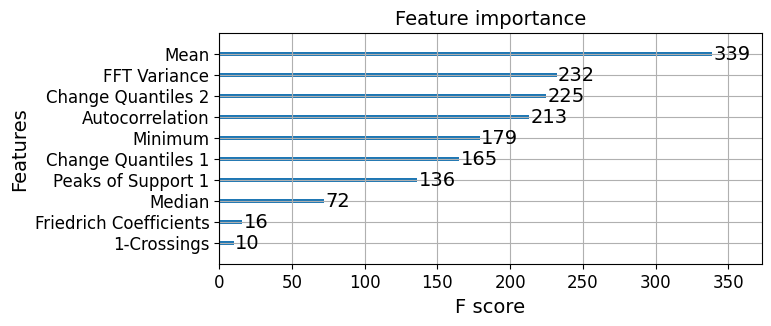
\includegraphics[width=\textwidth]{figures/classification/BH/BH-feature-selection.png}
% 		\caption{\textbf{Benjamini-Hochberg Feature Selection} for a set containing working and faulty sensors.}
% 		\label{fig:BH_feature_selection}
% 	\end{minipage}
% 	%%%%%%%%%%%%%%%%
% 	% END OF B-H FEATURE SELECTION
% 	%%%%%%%%%%%%%%%%
% 	\hspace{0.5ex}
%     \begin{subfigure}[t]{0.15\textwidth}
%         \centering
%         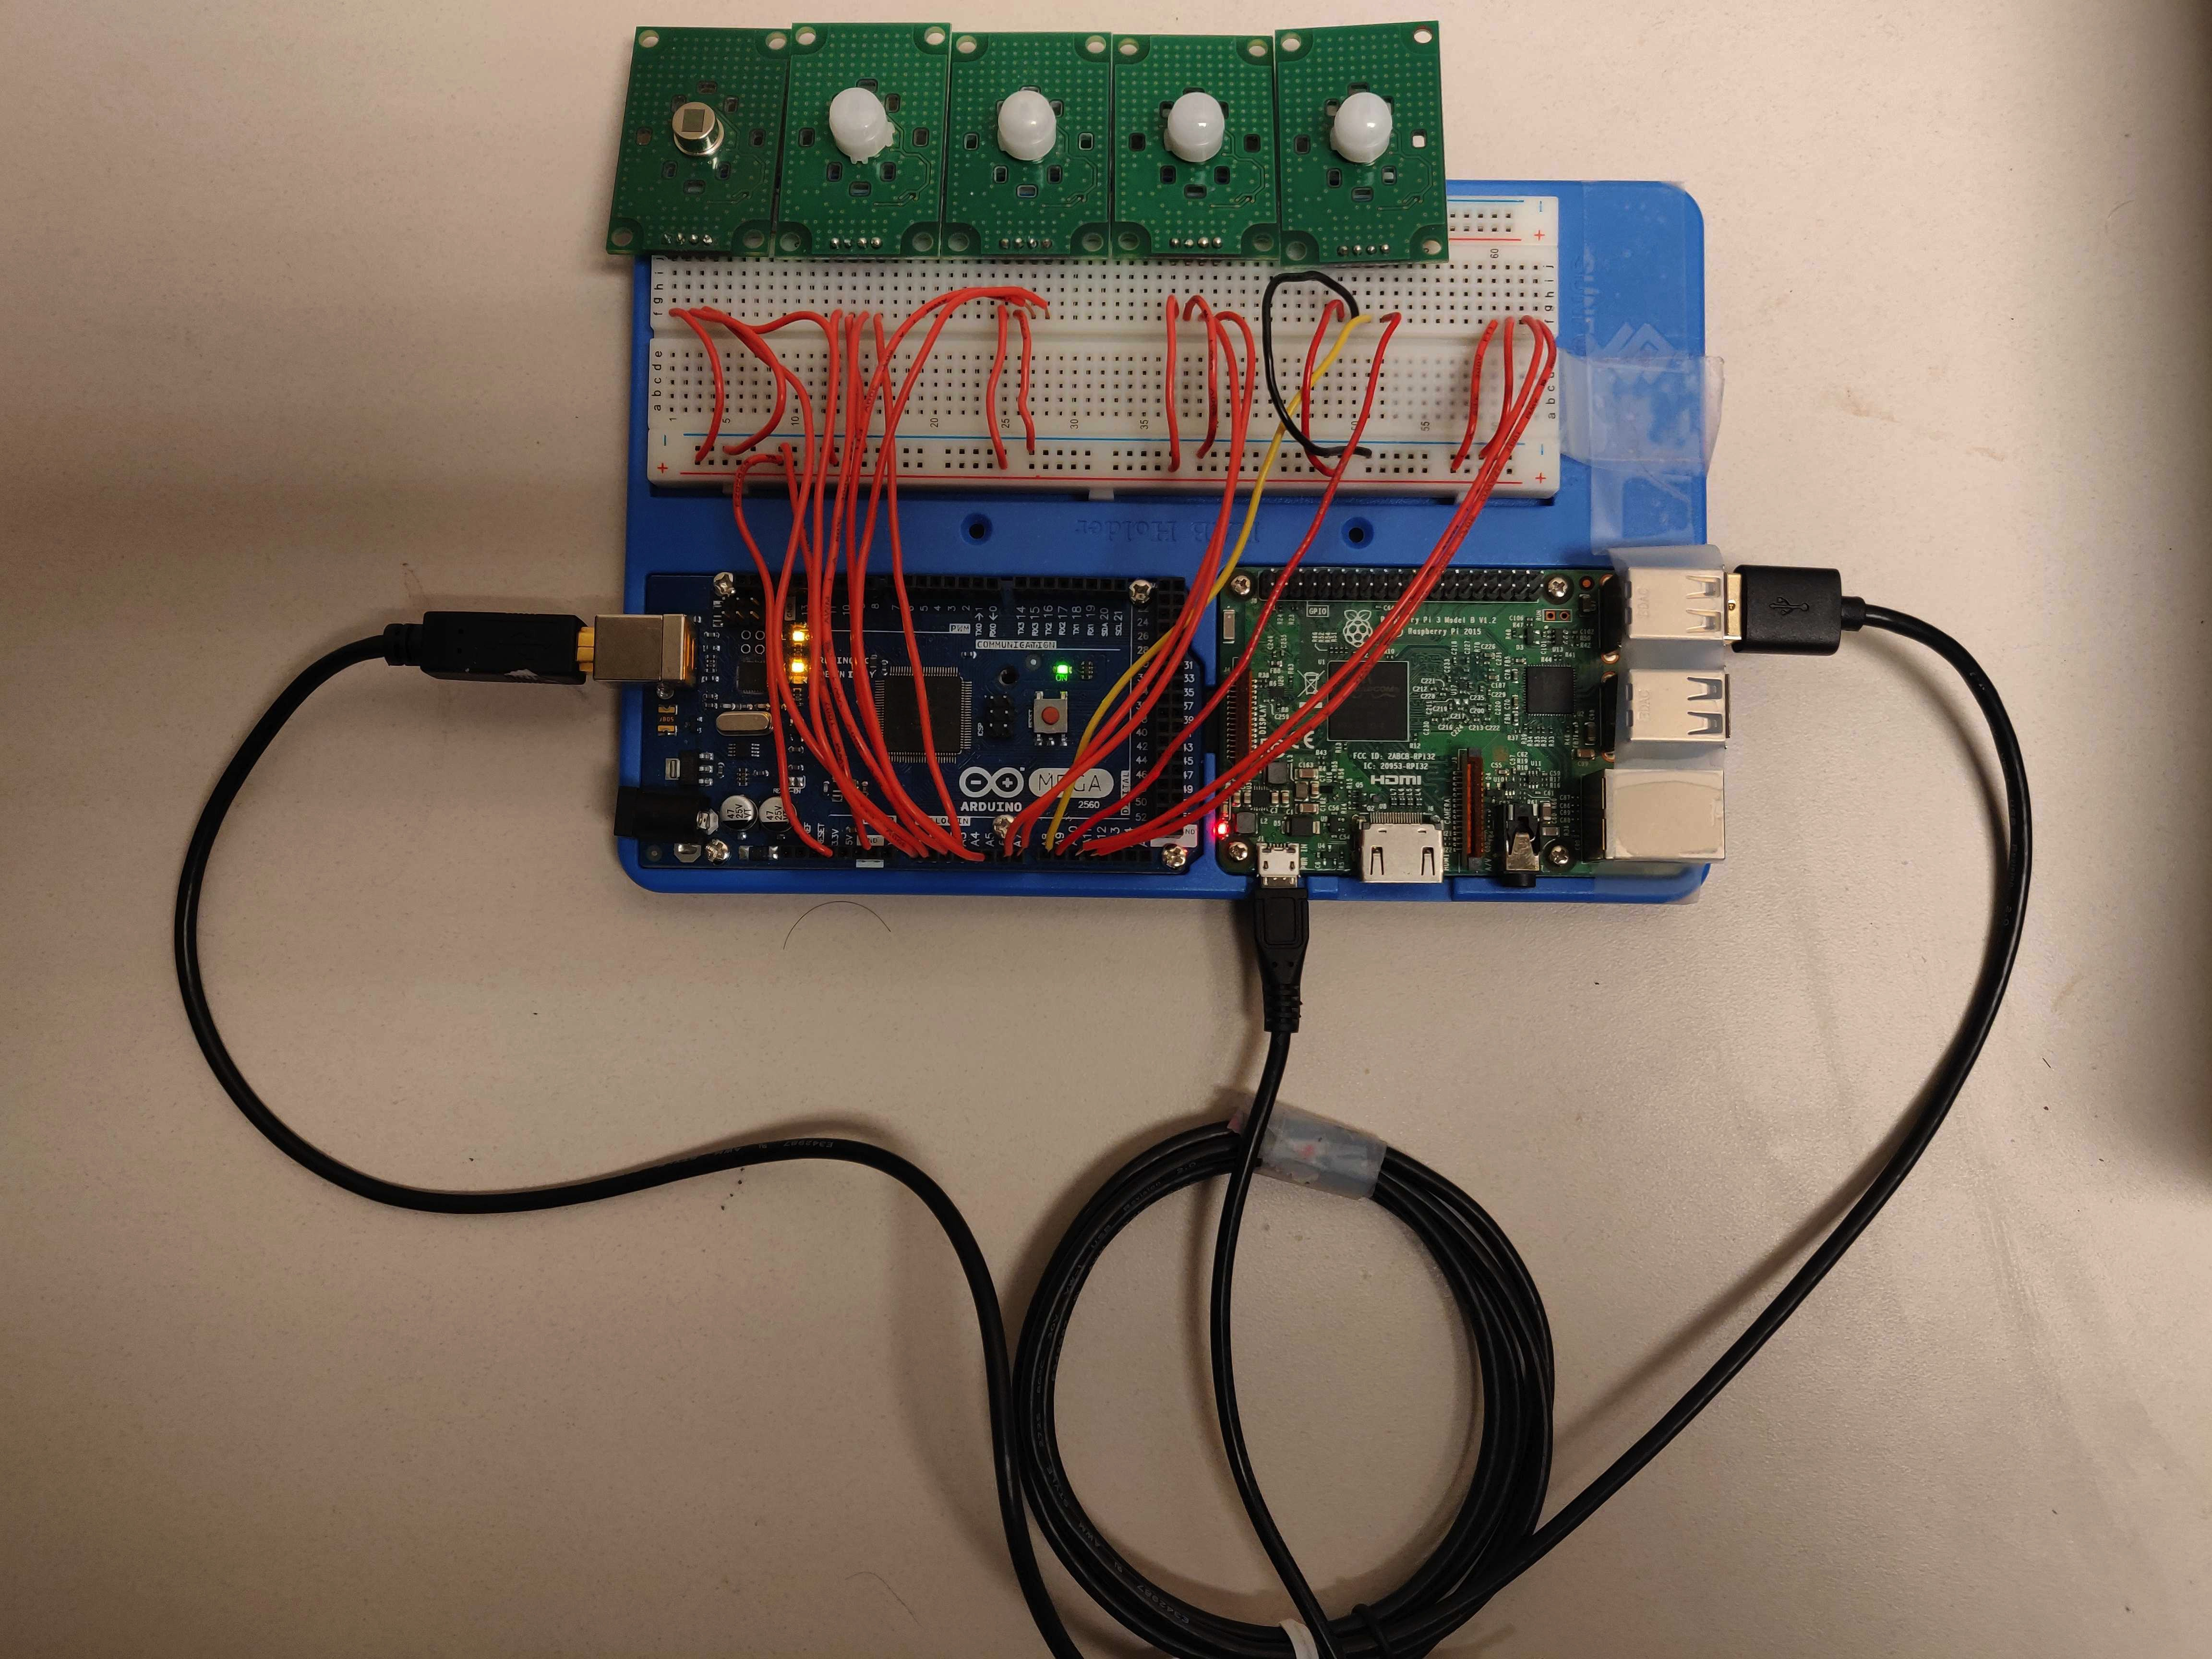
\includegraphics[width=\textwidth]{figures/platform/eval_platform.jpg}
%     \end{subfigure}
%	%%%%%%%%%%%%%%%
%	 ACCURACY VS WINDOW SIZE
%	%%%%%%%%%%%%%%%
%	\begin{subfigure}[t]{\textwidth}
%		 \centering
%		 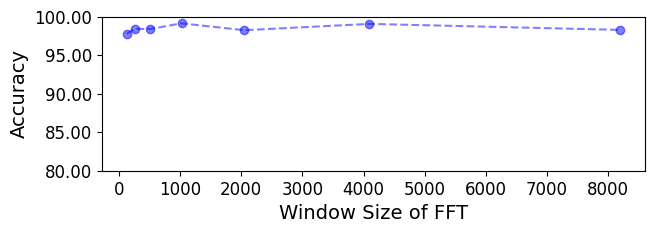
\includegraphics[width=0.4\textwidth, height=1.05in]{figures/classification/accuracy_vs_window_size.png}
%		 \caption{\footnotesize{Model Accuracy} for different window sizes. We choose 1024 as the default window size.}
%		 \label{fig:accuracy_vs_window_size}
%	\end{subfigure}
%	%%%%%%%%%%%%%%%
%	 END OF ACCURACY VS WINDOW SIZE
%	%%%%%%%%%%%%%%%
%\end{figure}
